\documentclass[journal]{IEEEtran}

\usepackage{graphicx}
\usepackage{float}
\usepackage{bm}
\usepackage{amsmath,amsfonts,amssymb,amsthm}
\usepackage{subcaption}
\usepackage{caption}

\usepackage{tex/macros}

\setlength{\abovecaptionskip}{10pt}
\captionsetup[figure]{
  font=small,
  % singlelinecheck?=f
}

\begin{document}

\title{Exploring Reservoir Computing with physical limits using Echo State Networks}
\author{Thomas Aven}
\date{}
\maketitle

\begin{abstract}
  Reservoir Computing (RC) emerged as an alternative framework to the
traditional gradient descent methods for training Recurrent Neural Networks
(RNNs). Key to the RC methodology is a randomly generated reservoir, commonly an
RNN that remains untrained, and a linear readout layer that is trained using
simple one-shot learning methods. Interestingly, there is no need for the
reservoir to be an artificial neural network -- any high-dimensional, driven
system exhibiting complex dynamic behavior can be used. A wide range of physical
reservoirs have been realized, ranging from optical laser circuits and
nanomagnetic assemblies to biological neural networks. The computational
performance of such physical substrates is closely related to common physical
limitations, e.g. noise, measurement accuracy, partially visible reservoir
state, and physical morphology. Here we investigate these fundamental properties
of physical reservoirs, offering insights into impairments that may be present
with such limitations, which in the wider context help improve the design of
future substrates.

% (TODO): concrete examples that help improve the design.

\end{abstract}

\begin{IEEEkeywords}
  Reservoir computing, unconventional computing, echo state networks, time
series computing.

  % (TODO): finish this list.

\end{IEEEkeywords}

%%% Local Variables:
%%% mode: latex
%%% TeX-master: "../main"
%%% End:

\section{Introduction}
Training Recurrent Neural Networks (RNNs) is an inherently difficult task
\cite{bengio_learning_1994}. To combat the high algorithmic complexity of
previous training methods, Echo State Networks (ESNs) \cite{jaeger_echo_2001}
present an alternative supervised learning technique that does not adapt the
internal weights of the network. Instead, the output is generated using a
simple, memoryless classifier or regressor, making the function of the internal
RNN resemble that of kernel methods. Thus, by projecting the input sequence into
a high-dimensional space, the temporal information of a time series may be
incorporated in the instantaneous readout. This methodology, concerned with
exploiting the underlying dynamics of a \textit{reservoir}, is unified in the
research subfield of Reservoir Computing (RC).

Interestingly, there is no need for the reservoir to be an artificial neural
network -- any high-dimensional, driven system exhibiting complex dynamic
behavior can be used \cite{schrauwen_overview_2007}. Reservoirs are thus
designed such that we are able to harness the dynamics that governs the
\textit{substrate} that implements it. A multitude of substrates have shown
promise as reservoirs: electronic memristor circuits
\cite{kulkarni_memristor-based_2012}, photonic systems
\cite{vandoorne_experimental_2014}, mechanical springs
\cite{hauser_towards_2011} and more biologically oriented reservoirs such as
gene regulation networks \cite{jones_is_2007} and the cat primary visual cortex
\cite{scholkopf_temporal_2007}. Consult \cite{tanaka_recent_2018} for an
overview of recent advances in physical RC.

In this paper we seek to investigate fundamental properties related to physical
reservoirs. Commonly, preliminary studies are conducted by simulating the
proposed dynamical system numerically to gauge its applicability in a physical
reservoir setting. Such models may not entirely encapsulate the uncertainties
and limitations that will exist in its corresponding physical setting, thus
leading to a divergence between the performances observed
\cite{vandoorne_experimental_2014, katumba_neuromorphic_2018,
  jensen_reservoir_2017}.

The extent of the performance degradation caused by physical limitations is not
readily understood. Hence, as implementations of reservoir systems increasingly
tend toward physical substrates, the computational performance may be affected
by intrinsic physical limitations such as noise, measurement equipment accuracy,
partially visible reservoir state, and physical morphology.

Reservoir robustness to noise is a primary concern that has been demonstrated
both numerically and experimentally in an optoeletronic setting, where
pre-processing techniques have been shown to reduce performance degradations
\cite{soriano_optoelectronic_2013}. It is well-established that ESNs are
resilient to internal noise \cite{jaeger_echo_2001}, but it is uncertain whether
this translates to intrinsically noisy inputs. ESNs provide a natural context
for studying the general significance of noise.

Another relevant noise characteristic is that of equipment
accuracy. Quantization noise, i.e. the resolution of the interface equipment, is
usually determined by DAC and ADC instruments. Employing equipment with
sufficient resolution has been found to be important when using physical
reservoirs \cite{soriano_delay-based_2015}.

Physical substrates will also differ in their process for both input
perturbation and state observation. The impact of input and output density,
i.e. the amount of reservoir nodes that are accessible to an observer, will
impact performance.

Lastly, being able to vary the input magnitude that each node sees freely is
desirable. Scaling the input signal before it is presented to the network is
usually easily accomplished, but applying individual weights for each internal
node is not, especially when considering a restrictive topology. Simple
weighting schemes, such as fixing all input weights to the same value, are of
interest.

The rest of this paper is structured as follows: first we provide relevant
background theory, including the motivation behind the exploration of each
physical limitation. Next we present methods and the simulation setup, followed
by a section on results and discussion. Finally we draw conclusions and suggest
future work.

%%% Local Variables:
%%% mode: latex
%%% TeX-master: "../main"
%%% End:

\section{Background}
\subsection{Echo State Networks}

The Echo State Network is a novel approach to training RNNs in which only the
weights of the output units are adapted \cite{jaeger_echo_2001}. Fig. \ref{esn}
illustrates the basic architecture of ESN reservoirs.

\begin{figure}[H]
  \centering
  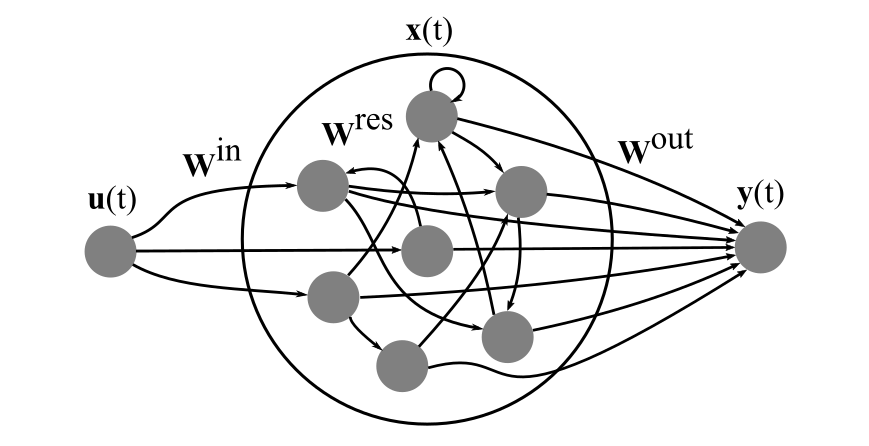
\includegraphics[width=2.5in]{img/esn.png}
  \caption{
    Basic architecture of ESN reservoir systems. The reservoir acts as a
high-dimensional kernel, transforming the temporal input sequence into a spatial
representation. The readout is trained with supervision, providing a least
squares optimum.
  }
  \label{esn}
\end{figure}

In the traditional ESN approach, the reservoir state is updated according to

\begin{equation}
  \mathbf{x}(t + 1) =
    \tanh(\mathbf{W}^{res}\mathbf{x}(t)
        + \mathbf{W}^{in}\mathbf{u}(t)),
  \label{xt}
\end{equation}

\noindent using $\tanh$ as the nonlinear transfer function for internal
reservoir nodes. The output of the reservoir is given by

\begin{equation}
  \mathbf{y}(t + 1) =
    \mathbf{W}^{out}\mathbf{x}(t).
  \label{yt}
\end{equation}

To train an ESN model of size N in a supervised and offline mode, it is run to
completion on a training set. The reservoir states are represented by an Nth
order column vector $\mathbf{X}$, and the one-dimensional output by a first
order column vector $\mathbf{Y}$. The linear readout layer is then trained to
minimize the squared output error $E = \norm{\mathbf{Y} - \mathbf{\hat{Y}}}$
where $\mathbf{\hat{Y}}$ is the target output, which amounts to finding the
$\mathbf{W}^{out}$ that minimizes this error with linear regression. Well-known
methods include ridge regression, often called Tikhonov regularization, and the
Moore-Penrose pseudo-inverse.

When the network is adapted to $\mathbf{W}^{out}$, the ESN is fully trained,
thus illustrating the apparent simplicity and low algorithmic complexity of the
method. Gauging the performance of a trained network is done by running a test
set. We use the normalized root mean square error (NRMSE) for this evaluation,
given a predicted signal $\mathbf{y}(t)$ and a target signal
$\mathbf{\hat{y}}(t)$

\begin{equation}
  E(\mathbf{y}, \mathbf{\hat{y}}) = \sqrt{\frac{
      \mean{\norm{\mathbf{y}(t) - \mathbf{\hat{y}}(t)}^{2}}
    }{
      \mean{\norm{\mathbf{\hat{y}}(t) - \mean{\mathbf{\hat{y}}(t)}}^{2}}
    }
  }
  .
  \label{nrmse}
\end{equation}

% I use NRMSE from Reservoir Computing Approaches to Recurrent Neural Network
% Training by Jaeger.

Applications of ESNs lie primarily in the domain of time series prediction and
classification, and the paradigm has been successfully applied to predict
myriads of benchmark time series \cite{goudarzi_comparative_2014,
alippi_quantification_2009, rodan_minimum_2011}. Real world approaches include
equalizing a wireless communication channel \cite{jaeger_harnessing_2004}, and
short-term traffic \cite{an_short-term_2011}, electric load
\cite{song_hourly_2011}, and stock price forecasting \cite{lin_short-term_2009}.

As with practically every machine learning technique, the application of ESNs
requires some experience. Although a conceptually simple idea, generating
adequate reservoir networks is influenced by multiple global
parameters. Parameters recommended to be of the most importance include the
scaling of the input weight matrix $\iota$, the spectral radius of the reservoir
connection matrix $\rho$, and the model size parameter $N$
\cite{montavon_practical_2012, jaeger_tutorial_nodate}.

\subsection{Assessing the quality of a reservoir}

In the RC methodology, computation and memory retainment are intertwined, in
stark contrast to traditional architectures which use separate memory storage
units. Attributing task-solving performance to either memory capacity or
computation is therefore quite difficult.

Attempts have been made to unify quality metrics for reservoir substrates,
e.g. the ability to separate different inputs \cite{legenstein_edge_2007}, the
ability to generalize \cite{legenstein_edge_2007}, and linear short-term memory
\cite{jaeger_short_2002}.

As we use extensively researched ESNs, we have chosen the NARMA10 time series to
be the main evaluation criteria for network performance. Its wide use enables
comparisons to previous work, which makes it a good candidate for evaluating
memory capacity and computational power with a single metric.

\subsection{NARMA}

Nonlinear autoregressive moving average (NARMA) \cite{atiya_new_2000},
\cite{kubota_dynamical_2019} is a class of time series models widely used to
benchmark the performance of RC models. We use the NARMA10 task to evaluate the
emulation performance of an ESN, which is a temporal task with a time-lag of ten
time steps, given by

% (TODO): Cite any NARMA users? Many listed in Kubota 2019^.

\begin{equation}
  y_{t+1} = \alpha y_{t} +
  \beta y_{t} \sum_{i=0}^{9}y_{t-i} +
  \gamma u_{t}u_{t-9} +
  \delta,
  \label{narma}
\end{equation}

\noindent with the default constant parameters $\alpha = 0.3$, $\beta = 0.05$,
$\gamma = 1.5$ and $\delta = 0.1$. The input $u_{t}$ is an i.i.d. stream drawn
from the interval [0, 0.5]. The task presents a challenge of both memory and
nonlinearity, uncovered to be a universal trade-off in in dynamical systems used
in reservoir settings \cite{dambre_information_2012, verstraeten_memory_2010},
therefore making it a well-suited task.

Evaluation of ESN performance on the NARMA10 system is a thoroughly explored
area in the field of RC, with the best NRMSE performances reported for
traditional ESN reservoirs of size $N = 200$ lying in the range [0.20, 0.25]
\cite{goudarzi_comparative_2014, rodan_minimum_2011,
verstraeten_experimental_2007, jaeger_adaptive_nodate}. For some context, using
a shift register containing the input as a reservoir will achieve a minimal
NRMSE of 0.4. To achieve NRMSE values below this threshold it is necessary to
introduce nonlinearity in the reservoir.

% (TODO): Introduce the problem statements individually for each
% limitation. ''Natural computational systems must have specific topologies, and
% the uniform random connectivity is not appropriate.'' Topology discussion,
% Manevitz et. al.

%%% Local Variables:
%%% mode: latex
%%% TeX-master: "../main"
%%% End:


\section{Physical limitations}
\subsection{Noise}

Physical, real world systems are affected by noise. By extension, designers of
reservoirs that use material substrates must be aware of the effects the noise
that is present may have on computational power.

It is well known in the field of traditional artificial neural networks that an
addition of noise to training data can lead to generalization improvements
similar to that of Tikhonov Regularization \cite{bishop_training_1995}. This has
been verified to hold for the RC paradigm \cite{jaeger_echo_2001,
kurkova_stable_2008}, where an additional noise term $\mathbf{v}(t)$ is added to
the reservoir. The noise is either added to all reservoir nodes, or to an output
\textit{feedback} of $\mathbf{y}(t)$ back into the reservoir nodes. A more
pragmatic approach is thus simply using ridge regression, as to avoid the
nondeterminism present with dynamic noise injection.

In the noise section we will investigate the impact of adding noise to just the
input signal, and hence exploring reservoir robustness to noisy environments.

Additive white Gaussian noise (AWGN) is a common noise model that mimics the
noise patterns of many random processes in nature. The noise is additive,
meaning the AWGN output is the sum of the input $u_{i}$ and the noise values
$v_{i}$. $v_{i}$ is i.i.d and drawn from a Gaussian distribution with zero-mean,
and a variance $\sigma^{2}$.

%%% Local Variables:
%%% mode: latex
%%% TeX-master: "../main"
%%% End:


\section{Methods}
All further reservoirs were constructed with the parameters from this baseline,
unless otherwise specified. The default reservoir size used was 200 hidden
nodes. $\mathbf{W}^{res}$ and $\mathbf{W}^{in}$ were both generated as random
matrices with i.i.d. entries in the interval [-0.5, 0.5]. Both matrices are
fully connected, and the reservoir weight matrix was rescaled such that
$\rho(\mathbf{W}_{res}) = 0.9$. The first 200 states of each run are discarded
to provide a \textit{washout} of the initial reservoir state. For all
experiments, the generated input was split into a training and test set, with
$L_{train} = 2000$ and $L_{test} = 3000$. All reported performances are the mean
across ten randomizations of each model representative. The Python software
library implementation is available online\footnote{Some GitHub repository.}.

\subsection{Noise}

We model AWGN by extending the ESN model to take the sum of two individual
inputs, $\mathbf{u}(t)$ and $\mathbf{v}(t)$, which represent the signal and the
noise. The goal of the reservoir remains a computation on the signal
$\mathbf{u}(t)$, a task now hindered by the unwanted noise. The ESN reservoirs
used are of size $N = 200$.

We vary the signal to noise ratio of the injected noise when running the test
dataset. The signal to noise ratio is measured in dB, and is calculated as $SNR
= 10\log_{10}(\frac{var(u)}{var(v)})$. The results are shown in
Fig. \ref{input_noise_snr}, illustrating a slight performance degradation when
the ratio of signal power to noise power drops below 20 dB. The reservoir
performance drops more drastically when reaching 10 dB. Similar performance
degradation was seen in \cite{dambre_information_2012}, where the same SNR
measure was used to evaluate the signal reconstruction capacity from the state
of a dynamical system.

\begin{figure}
  \centering
  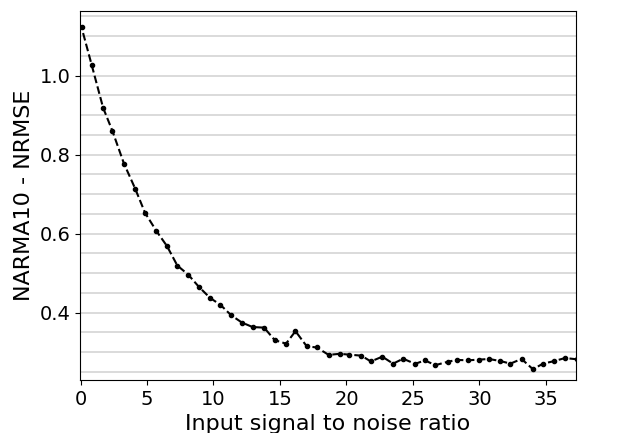
\includegraphics[width=2.5in]{img/input_noise_snr.png}
  \caption{
    Noise causing a decrease in performance for an ESN reservoir on the NARMA10
task ($N = 200$ nodes). When the signal to noise ratio drops below 20dB, the
performance of the reservoir degrades in an exponential manner.
  }
  \label{input_noise_snr}
\end{figure}

\subsection{Measurement equipment accuracy}

To emulate the behavior of an ADC, we extend our ESN model to allow for
quantization of reservoir output before it is passed to the readout layer. This
quantization effectively divides the range of the nonlinear activation function
of each hidden node into a discrete set of fixed output bins.

\begin{figure}[H]
  \centering
  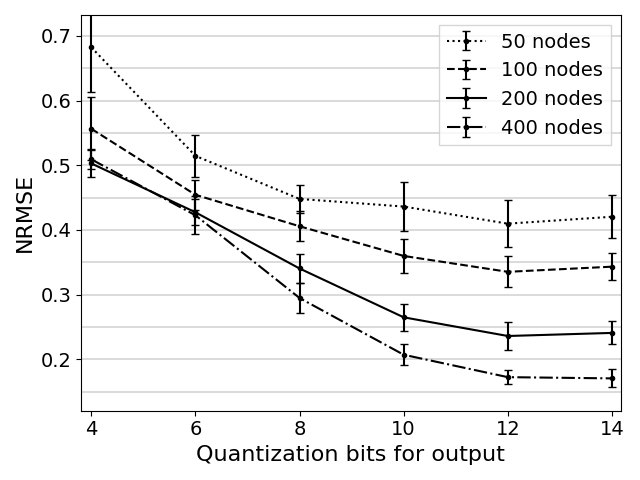
\includegraphics[width=2.5in]{img/adc_quantization.png}
  \caption{
    Performance effect of ADC quantization on four reservoirs of different
sizes. $\tanh$ is used as activation function for the experiment, dividing its
range of (1-, 1) into $n$ discrete output bins.
  }
  \label{adc_quantization}
\end{figure}

% (TODO): Change this to bits of quantization? As if it's an actual ADC.

Fig. \ref{adc_quantization} shows how quantization affects reservoir
performance. We plot the error of four different reservoir sizes: 50, 100, 200
and 400 hidden nodes to see whether it is possible to compensate for lower
resolutions by increasing the size of the reservoir.

\subsection{Partially visible reservoir state}

\begin{figure*}[htbp]
  \centering
  \begin{subfigure}{.3\textwidth}
    \centering
    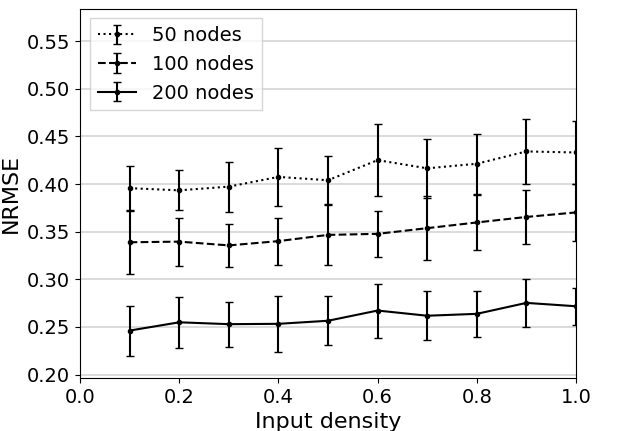
\includegraphics[width=\linewidth]{img/input_density_all.png}
    \caption{}
  \end{subfigure}
  \begin{subfigure}{.3\textwidth}
    \centering
    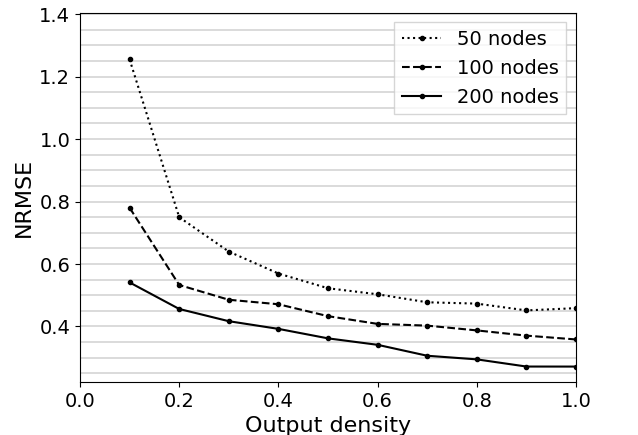
\includegraphics[width=\linewidth]{img/output_density_all.png}
    \caption{}
  \end{subfigure}
  \begin{subfigure}{.3\textwidth}
    \centering
    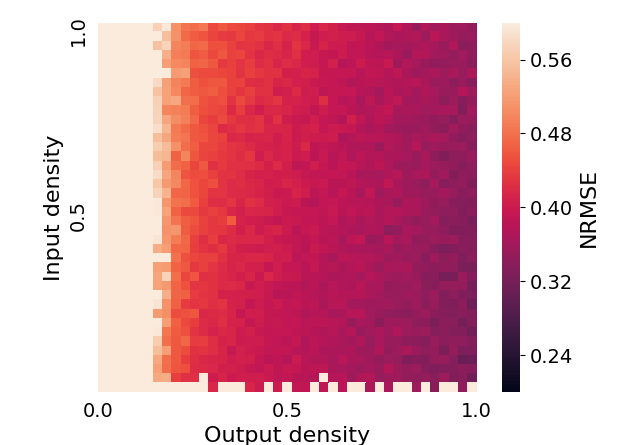
\includegraphics[width=\linewidth]{img/partial_visibility.png}
    \caption{}
  \end{subfigure}
  \caption{
    These figures show the influence of reservoirs that are only partially
visible on the performance for the NARMA10 task. The density is a measurement
for the fraction of elements in the input and output matrices containing
non-zero elements. The heat map was generated using a reservoir size of 200
hidden nodes.
  }
  \label{partial_visibility}
\end{figure*}

We begin by experimenting with the sparsity of $\mathbf{W}_{in}$ and
$\mathbf{W}_{out}$. In both cases, we now generate the connection matrices such
that a wanted density, given as the fraction of connected nodes, is
achieved. Input and output is adjusted separately. Fig. \ref{partial_visibility}
shows the results of our simulation runs.

\begin{figure}[H]
  \centering
  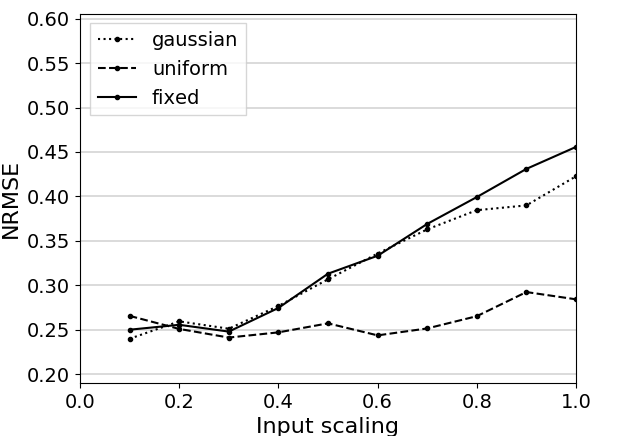
\includegraphics[width=2.5in]{img/input_scaling_distrib.png}
  \caption{
    Effect of input scaling on three input weight distributions. With the fixed
distribution every input weight is set to 1. The best performance of all three
distributions lie around NRMSE $\approx 0.25$.
  }
  \label{input_scaling_distrib}
\end{figure}

Additionally, we examine three different input weight distributions: uniform,
Gaussian and fixed. All inputs are all sampled as i.i.d streams. The uniform
distribution is sampled in the interval [-0.5, 0.5], the Gaussian distribution
is sampled with a zero mean and standard deviation $\sigma = 1.0$, and the fixed
distribution has every input weight set to 1. Moreover, we explore the parameter
space of the input scaling in the interval [0.1, 1.0].

%%% Local Variables:
%%% mode: latex
%%% TeX-master: "../main"
%%% End:


\section{Results and discussion}
Evaluation of ESN performance on the NARMA system is a thoroughly explored area
in the field of RC \cite{verstraeten_experimental_2007, rodan_minimum_2011,
jaeger_adaptive_nodate}. Similar performance to previous work has been achieved
(Fig. \ref{performance}) lending credibility to further approaches in this
paper.

\begin{figure}[H]
  \centering
  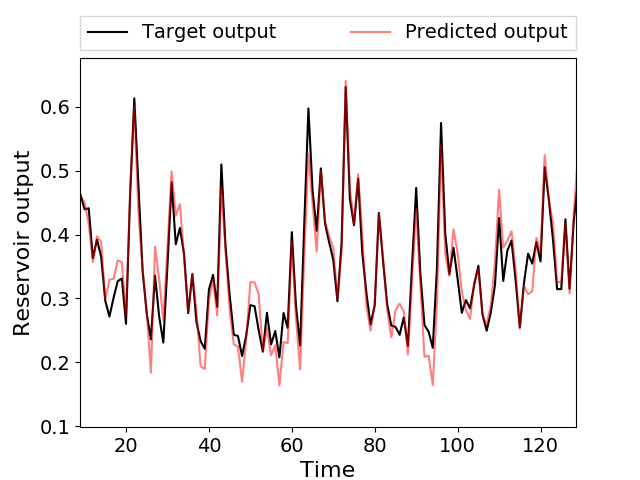
\includegraphics[width=2.5in]{img/narma_visualization.png}
  \caption{
    Visualization of reservoir output. (TODO): Re-do this screenshot so it's
possible to see anything at all.
  }
  \label{visualization}
\end{figure}

\begin{figure}[H]
  \centering
  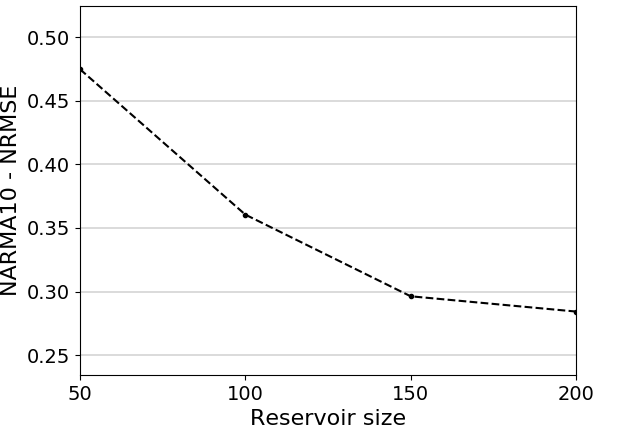
\includegraphics[width=2.5in]{img/general_performance.png}
  \caption{
    ESN performance. Performed with input scaling of 1, spectral radius 0.9,
input sparsity of 1.0, no leaky nodes. 10 random reservoirs were sampled for
each reservoir size.
  }
  \label{performance}
\end{figure}
% (TODO): Fix caption to suck less for both of these^.

\subsection{Noise}

\subsection{Measurement equipment accuracy}

\subsection{Partial visible state}

\subsection{Topology}


% Thoughts
% * Remember to add NRMSE to heatmap plots.

%%% Local Variables:
%%% mode: latex
%%% TeX-master: "../main"
%%% End:


\section{Conclusion}
Conclusion.


%%% Local Variables:
%%% mode: latex
%%% TeX-master: "../main"
%%% End:


\section{Future work}
Further investigations is inclined to be of twofold nature. First, it is ...

\subsection{What if nodes are dying? Binary vs. non-binary}

\subsection{Topology and physical morphology}

%%% Local Variables:
%%% mode: latex
%%% TeX-master: "../main"
%%% End:


\bibliography{ref.bib}
\bibliographystyle{ieeetr}

\end{document}

%%% Local Variables:
%%% mode: latex
%%% TeX-master: t
%%% End:
